\documentclass[12pt,a4paper]{extarticle}
\usepackage[utf8]{inputenc}
\usepackage[T5]{fontenc}
\usepackage{geometry}
\geometry{a4paper, left=1.5cm, right=1cm, top=1.5cm, bottom=1.5cm, headheight=20pt, headsep=15pt, footskip=28pt}
\usepackage{enumitem}
\usepackage{amsmath}
\usepackage{amssymb}
\usepackage{diagbox}
\usepackage{colortbl} % Sửa lỗi \arrayrulecolor
\usepackage{array}    % Hỗ trợ định dạng cột m{2cm}
\usepackage[most]{tcolorbox}
\newcommand{\khongxacdinh}{\text{KXĐ}}
\newcommand{\blackbox}[1]{\texorpdfstring{\fcolorbox{black}{black}{\textcolor{white}{#1}}}{#1}}
\usepackage{tikz}
\definecolor{bookblue}{RGB}{58,90,172}
\definecolor{book}{RGB}{58,90,172}
\definecolor{myblue}{RGB}{200,40,40}
\newcommand{\bluecheck}{\textcolor{myblue}{\checkmark}}
\newtcolorbox{formulaBox}{colback=gray!5,colframe=bookblue,boxrule=0.8pt,arc=2mm}
\newtcolorbox{notebox}{colback=blue!3,colframe=myblue,boxrule=0.8pt,arc=2mm}
\usetikzlibrary{patterns, patterns.meta} % Thêm patterns.meta vào đây
% Gọi package nằm trong thư mục con template
\usepackage{../template/mngocbox}

\begin{document}

% Sử dụng ngoặc vuông [...] để thay đổi linh hoạt các thông số
\makeheadbox[headerright={Chương 2},chude={Bài 1},tieude={Vector cơ bản},dinhdang={Hình học},lop={12 },gv={Nguyễn Lê Minh Ngọc}]
\vspace{2em}
\makeheading{I}{Kiến thức cần nhớ}



\section*{A. KIẾN THỨC CẦN NHỚ}
\subsection*{I. Ôn lại}
\begin{enumerate}[label=\arabic*., leftmargin=*, itemsep=1.5em]
    % 1. Khái niệm vectơ
    \item \textbf{Khái niệm vectơ} (vectơ là $1$ đoạn thẳng có hướng)
    \begin{center}
        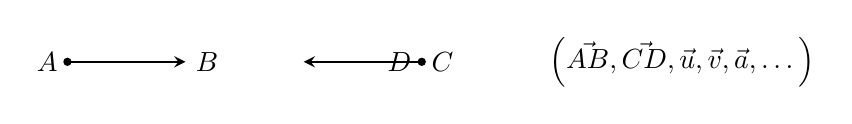
\begin{tikzpicture}[scale=1.0, >=stealth]
            \fill (0,0) circle (1.5pt) node[left] {$A$};
            \draw[->, thick] (0,0) -- (1.5,0) node[right] {$B$};
            
            \fill (4.5,0) circle (1.5pt) node[right] {$C$};
            \draw[<-, thick] (3.0,0) -- (4.5,0) node[left] {$D$};
            
            \node[right=1cm] at (5.0,0) {$\left(\vec{AB}, \vec{CD}, \vec{u}, \vec{v}, \vec{a}, \dots\right)$};
        \end{tikzpicture}
    \end{center}
    % 2. Giá của vectơ
    \item \textbf{Giá của vectơ}
    \begin{center}
        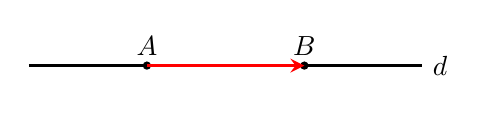
\begin{tikzpicture}[scale=1.0, >=stealth]
            \draw[thick] (-1.0,0) -- (4.0,0) node[right] {$d$};
            \fill (0.5,0) circle (1.5pt) node[above] {$A$};
            \fill (2.5,0) circle (1.5pt) node[above] {$B$};
            \draw[->, red, very thick] (0.5,0) -- (2.5,0);
        \end{tikzpicture}
    \end{center}
    % 3. Độ dài vectơ
    \item \textbf{Độ dài vectơ:} \quad $\left|\vec{AB}\right| = AB$
    % 4. Hai vectơ cùng phương
    \item \textbf{Hai vectơ cùng phương}
    \begin{center}
        \begin{minipage}{0.45\textwidth}
            \centering
            % Hai đường thẳng song song
            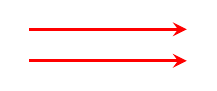
\begin{tikzpicture}[scale=1.0, >=stealth]
                \draw[->, red, very thick] (0,0.4) -- (2.0,0.4);
                \draw[->, red, very thick] (0,0) -- (2.0,0);
            \end{tikzpicture}
            \par\vspace{0.1cm} \small Song song
        \end{minipage}
        \hfill
        \begin{minipage}{0.45\textwidth}
            \centering
            % Trùng nhau (cùng nằm trên một đường thẳng)
            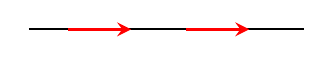
\begin{tikzpicture}[scale=1.0, >=stealth]
                \draw[thick] (-0.5,0) -- (3.0,0);
                \draw[->, red, very thick] (0,0) -- (0.8,0);
                \draw[->, red, very thick] (1.5,0) -- (2.3,0);
            \end{tikzpicture}
            \par\vspace{0.1cm} \small Trùng nhau (cùng nằm trên đường thẳng)
        \end{minipage}
    \end{center}
    % 5. Hai vectơ cùng hướng
    \item \textbf{Hai vectơ cùng hướng}
    \begin{center}
        \begin{minipage}{0.45\textwidth}
            \centering
            
\begin{tikzpicture}[scale=1.0, >=stealth]
                \draw[->, thick] (0,0.4) -- (1.5,0.4);
                \draw[->, thick] (0,0) -- (1.5,0);
                \draw[red, thick] (2.2,0.2) circle (8pt) node {\checkmark};
            \end{tikzpicture}
            \par\vspace{0.1cm} \small Cùng hướng
        \end{minipage}
        \hfill
        \begin{minipage}{0.45\textwidth}
            \centering
            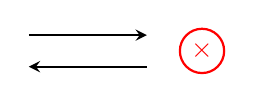
\begin{tikzpicture}[scale=1.0, >=stealth]
                \draw[->, thick] (0,0.4) -- (1.5,0.4);
                \draw[<-, thick] (0,0) -- (1.5,0);
                \draw[red, thick] (2.2,0.2) circle (8pt) node {$\times$};
            \end{tikzpicture}
            \par\vspace{0.1cm} \small Ngược hướng
        \end{minipage}
    \end{center}
    % 6. Hai vectơ bằng nhau
    \item \textbf{Hai vectơ bằng nhau:} \quad cùng hướng và cùng độ dài
    \begin{center}
        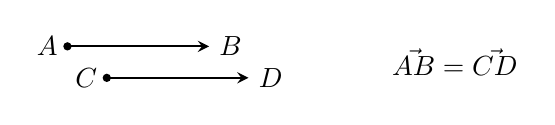
\begin{tikzpicture}[scale=1.0, >=stealth]
            \fill (0,0.4) circle (1.5pt) node[left] {$A$};
            \draw[->, thick] (0,0.4) -- (1.8,0.4) node[right] {$B$};
            
            \fill (0.5,0) circle (1.5pt) node[left] {$C$};
            \draw[->, thick] (0.5,0) -- (2.3,0) node[right] {$D$};
            
            \node[right=1.5cm] at (2.5,0.2) {$\vec{AB} = \vec{CD}$};
        \end{tikzpicture}
    \end{center}
    % 7. Hai vectơ đối nhau
    \item \textbf{Hai vectơ đối nhau:} \quad ngược hướng và cùng độ dài
    \begin{center}
        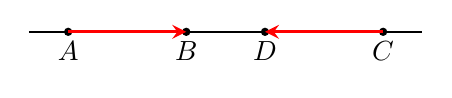
\begin{tikzpicture}[scale=1.0, >=stealth]
            \draw[thick] (-0.5,0) -- (4.5,0);
            \fill (0,0) circle (1.5pt) node[below] {$A$};
            \fill (1.5,0) circle (1.5pt) node[below] {$B$};
            \fill (2.5,0) circle (1.5pt) node[below] {$D$};
            \fill (4.0,0) circle (1.5pt) node[below] {$C$};
            
            \draw[->, red, very thick] (0,0) -- (1.5,0);
            \draw[<-, red, very thick] (2.5,0) -- (4.0,0); % Vec(CD) ngược hướng Vec(AB)
        \end{tikzpicture}
    \end{center}
    % 8. Vectơ-không
    \item \textbf{Vectơ-không:} \quad $\vec{0}$, \quad điểm đầu $\equiv$ điểm cuối
    \[
    \vec{AA} = \vec{0}
    \]
    % 9. Tổng của 2 vectơ
    \item \textbf{Tổng của 2 vectơ} (Quy tắc tam giác)
    \begin{center}
        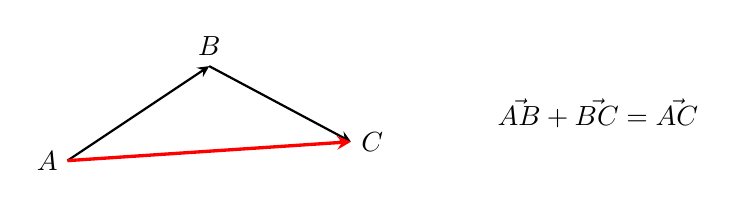
\begin{tikzpicture}[scale=1.2, >=stealth]
            \coordinate (A) at (0,0);
            \coordinate (B) at (1.5,1.0);
            \coordinate (C) at (3.0,0.2);
            
            \draw[->, thick] (A) -- (B) node[above] {$B$};
            \draw[->, thick] (B) -- (C) node[right] {$C$};
            \draw[->, red, very thick] (A) -- (C);
            
            \node[left] at (A) {$A$};
            
            \node[right=1.5cm] at (3.2,0.5) {$\vec{AB} + \vec{BC} = \vec{AC}$};
        \end{tikzpicture}
    \end{center}
\end{enumerate}
    % 10. Quy tắc hình bình hành
    \item \textbf{Quy tắc hình bình hành}
    \begin{center}
        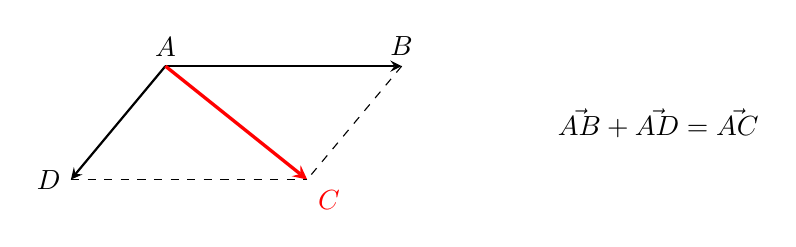
\begin{tikzpicture}[scale=1.2, >=stealth]
            \coordinate (A) at (1.0,1.2);
            \coordinate (B) at (3.5,1.2);
            \coordinate (D) at (0,0);
            \coordinate (C) at (2.5,0);
            
            \draw[->, thick] (A) -- (B) node[above] {$B$};
            \draw[->, thick] (A) -- (D) node[left] {$D$};
            \draw[->, red, very thick] (A) -- (C) node[below right] {$C$};
            
            \draw[dashed] (B) -- (C);
            \draw[dashed] (D) -- (C);
            
            \node[above] at (A) {$A$};
            
            \node[right=1.5cm] at (3.8,0.6) {$\vec{AB} + \vec{AD} = \vec{AC}$};
        \end{tikzpicture}
    \end{center}

    % 11. Phép trừ hai vectơ
    \item \textbf{Phép trừ hai vectơ:}
    \[
    \vec{AB} - \vec{AC} = \vec{AB} + \vec{CA} = \vec{CA} + \vec{AB} = \vec{CB}
    \]

    % 12. Tính chất phép cộng
    \item \textbf{Tính chất phép cộng:} Cho 3 vectơ $\vec{a}, \vec{b}, \vec{c}$ bất kỳ.
    \begin{itemize}[label=$\bullet$, leftmargin=1.5cm, itemsep=0.3em]
        \item Giao hoán: $\vec{a} + \vec{b} = \vec{b} + \vec{a}$
        \item Kết hợp: $(\vec{a} + \vec{b}) + \vec{c} = \vec{a} + (\vec{b} + \vec{c})$
        \item Cộng vectơ-không: $\vec{a} + \vec{0} = \vec{a}$
    \end{itemize}

    % 13. Tích của vectơ với 1 số
    \item \textbf{Tích của vectơ với 1 số}
    \par Cho $k \neq 0$ ($k \in \mathbb{R}$) và $\vec{a} \neq \vec{0}$. Tích của vectơ $\vec{a}$ với số thực $k$, ký hiệu $k\vec{a}$, được xác định bởi:
    \begin{center}
        \begin{minipage}{0.48\textwidth}
            \centering
            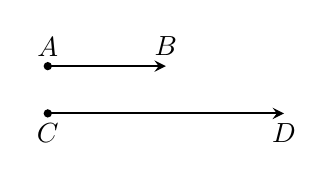
\begin{tikzpicture}[scale=1.0, >=stealth]
                \fill (0,0.5) circle (1.5pt) node[above] {$A$};
                \draw[->, thick] (0,0.5) -- (1.5,0.5) node[above] {$B$};
                
                \fill (0,-0.1) circle (1.5pt) node[below] {$C$};
                \draw[->, thick] (0,-0.1) -- (3.0,-0.1) node[below] {$D$};
            \end{tikzpicture}
            \par\vspace{0.1cm}
            $\left(\vec{CD} = 2\vec{AB}\right)$
        \end{minipage}
        \hfill
        \begin{minipage}{0.48\textwidth}
            \begin{itemize}[label=$\bullet$, leftmargin=*, itemsep=0.3em]
                \item Cùng hướng $\vec{a}$ nếu $k > 0$.
                \item Ngược hướng $\vec{a}$ nếu $k < 0$.
                \item Độ dài bằng $|k| \cdot |\vec{a}|$.
            \end{itemize}
        \end{minipage}
    \end{center}
    \textbf{Quy ước:} $0 \cdot \vec{a} = \vec{0}$ và $k \cdot \vec{0} = \vec{0}$.

    % 14. Tính chất của tích vectơ với 1 số
    \item \textbf{Tính chất của tích vectơ với 1 số:} Cho $\vec{a}, \vec{b}$ là 2 vectơ bất kỳ và 2 số thực $h, k$.
    \begin{center}
        \begin{tabular}{ll}
            $k(\vec{a} + \vec{b}) = k\vec{a} + k\vec{b}$ & $k(\vec{a} - \vec{b}) = k\vec{a} - k\vec{b}$ \\[0.3em]
            $(h + k)\vec{a} = h\vec{a} + k\vec{a}$ & $h(k\vec{a}) = (hk)\vec{a}$ \\[0.3em]
            $1 \cdot \vec{a} = \vec{a}$ & $(-1)\vec{a} = -\vec{a}$
        \end{tabular}
    \end{center}

    % 15. Công thức trung điểm
    \item \textbf{Công thức trung điểm}
    \begin{center}
        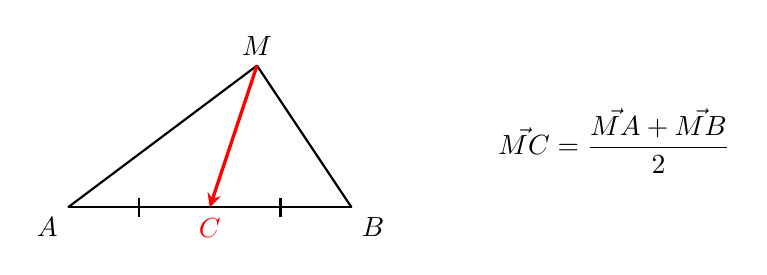
\begin{tikzpicture}[scale=1.2, >=stealth]
            \coordinate (A) at (0,0);
            \coordinate (B) at (3.0,0);
            \coordinate (C) at (1.5,0);
            \coordinate (M) at (2.0,1.5);
            
            \draw[thick] (A) -- (B);
            \draw[thick] (M) -- (A) node[below left] {$A$};
            \draw[thick] (M) -- (B) node[below right] {$B$};
            \draw[->, red, very thick] (M) -- (C) node[below] {$C$};
            
            \node[above] at (M) {$M$};
            
            % Kí hiệu đoạn thẳng bằng nhau
            \draw[thick] (0.75,-0.1) -- (0.75,0.1);
            \draw[thick] (2.25,-0.1) -- (2.25,0.1);
            
            \node[right=1.5cm] at (3.2,0.7) {$\vec{MC} = \dfrac{\vec{MA} + \vec{MB}}{2}$};
        \end{tikzpicture}
    \end{center}
        % 16. Công thức trọng tâm của tam giác
    \item \textbf{Công thức trọng tâm của tam giác}
    \par Gọi $G$ là trọng tâm $\triangle ABC$ và $M$ là $1$ điểm bất kỳ (lưu ý: $M$ bất kỳ trong không gian).
    \begin{center}
        \begin{minipage}{0.4\textwidth}
            \centering
            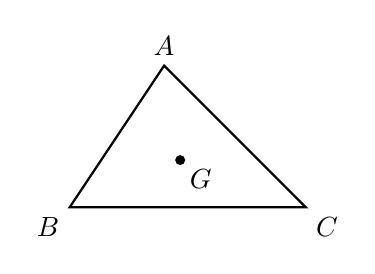
\begin{tikzpicture}[scale=1.2, >=stealth]
                \coordinate (A) at (1.0,1.5);
                \coordinate (B) at (0,0);
                \coordinate (C) at (2.5,0);
                
                \draw[thick] (A) -- (B) node[below left] {$B$} -- (C) node[below right] {$C$} -- cycle;
                \node[above] at (A) {$A$};
                
                \coordinate (G) at (1.17,0.5);
                \fill (G) circle (1.5pt) node[below right] {$G$};
            \end{tikzpicture}
        \end{minipage}
        \hfill
        \begin{minipage}{0.55\textwidth}
            \begin{itemize}[label=$\bullet$, leftmargin=*]
                \item $\vec{GA} + \vec{GB} + \vec{GC} = \vec{0}$
                \item $\vec{MA} + \vec{MB} + \vec{MC} = 3\vec{MG}$
            \end{itemize}
        \end{minipage}
    \end{center}
    \textbf{Chứng minh:}
    \[
    \begin{cases}
        \vec{MA} = \vec{MG} + \vec{GA} \\
        \vec{MB} = \vec{MG} + \vec{GB} \\
        \vec{MC} = \vec{MG} + \vec{GC}
    \end{cases}
    \implies \vec{MA} + \vec{MB} + \vec{MC} = 3\vec{MG} + \underbrace{(\vec{GA} + \vec{GB} + \vec{GC})}_{\vec{0}} = 3\vec{MG}
    \]

    % 17. Tích vô hướng của hai vectơ
    \item \textbf{Tích vô hướng của hai vectơ}
    \par Góc giữa hai vectơ $\vec{a}$ và $\vec{b}$, ký hiệu $(\vec{a}, \vec{b}) = \alpha$ với $0^\circ \le \alpha \le 180^\circ$.
    \begin{center}
        \begin{minipage}{0.48\textwidth}
            \centering
            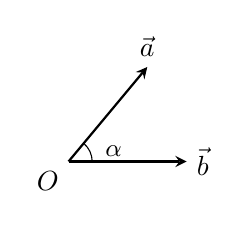
\begin{tikzpicture}[scale=1.0, >=stealth]
                \coordinate (O) at (0,0);
                \draw[->, thick] (O) -- (1.5,0) node[right] {$\vec{b}$};
                \draw[->, thick] (O) -- (1.0,1.2) node[above] {$\vec{a}$};
                \draw (0.3,0) arc (0:50:0.3) node[midway, right=2pt, font=\small] {$\alpha$};
                \node[below left] at (O) {$O$};
            \end{tikzpicture}
            \par\vspace{0.1cm} \small Góc nhọn $\alpha < 90^\circ$
        \end{minipage}
        \hfill
        \begin{minipage}{0.48\textwidth}
            \centering
            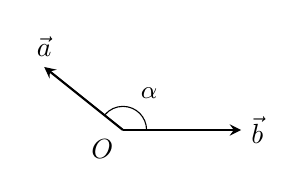
\begin{tikzpicture}[scale=1.0, >=stealth]
                \coordinate (O) at (0,0);
                \draw[->, thick] (O) -- (1.5,0) node[right] {$\vec{b}$};
                \draw[->, thick] (O) -- (-1.0,0.8) node[above] {$\vec{a}$};
                \draw (0.3,0) arc (0:140:0.3) node[midway, above right, font=\small] {$\alpha$};
                \node[below left] at (O) {$O$};
            \end{tikzpicture}
            \par\vspace{0.1cm} \small Góc tù $\alpha > 90^\circ$
        \end{minipage}
    \end{center}
    Công thức định nghĩa tích vô hướng:
    \[
    \boxed{\vec{a} \cdot \vec{b} = |\vec{a}| \cdot |\vec{b}| \cdot \cos(\vec{a}, \vec{b})}
    \]

    % 18. Tính chất của tích vô hướng
    \item \textbf{Tính chất của tích vô hướng:} Cho $\vec{a}, \vec{b}, \vec{c}$ là các vectơ bất kỳ và $k \in \mathbb{R}$.
    \begin{itemize}[label=$\bullet$, leftmargin=1.5cm, itemsep=0.4em]
        \item Giao hoán: $\vec{a} \cdot \vec{b} = \vec{b} \cdot \vec{a}$
        \item Phân phối: $\vec{a}(\vec{b} + \vec{c}) = \vec{a}\cdot\vec{b} + \vec{a}\cdot\vec{c}$
        \item Kết hợp với số thực: $(k\vec{a}) \cdot \vec{b} = k(\vec{a} \cdot \vec{b}) = \vec{a} \cdot (k\vec{b})$
        \item Bình phương vô hướng: $\vec{a}^2 = |\vec{a}|^2$
        \par\textit{(Vì $\vec{a} \cdot \vec{a} = |\vec{a}| \cdot |\vec{a}| \cdot \cos(\vec{a}, \vec{a}) = |\vec{a}|^2 \cdot \cos 0^\circ = |\vec{a}|^2$)}
        \item Bình phương đoạn thẳng: $\vec{AB}^2 = |\vec{AB}|^2 = AB^2$
    \end{itemize}

    % 19. Một số hệ thức cần lưu ý
    \item \textbf{Một số hệ thức cần lưu ý}
    \par Cho $\triangle ABC$:
    \[
    \vec{AB} \cdot \vec{AC} = \frac{1}{2}\left(AB^2 + AC^2 - BC^2\right)
    \]
    \textbf{Giải thích:}
    \begin{align*}
        BC^2 = \vec{BC}^2 &= \left(\vec{AC} - \vec{AB}\right)^2 \\
        &= \vec{AC}^2 + \vec{AB}^2 - 2\vec{AC} \cdot \vec{AB} \\
        &= AC^2 + AB^2 - 2\vec{AC} \cdot \vec{AB} \\
        \implies \vec{AC} \cdot \vec{AB} &= \frac{1}{2}\left(AC^2 + AB^2 - BC^2\right)
    \end{align*}
        % 20. Công thức đường trung tuyến
    \item \textbf{Công thức đường trung tuyến}
    \par Cho $\triangle ABC$ có $AM$ là trung tuyến ($BM = MC$).
    \begin{center}
        \begin{minipage}{0.4\textwidth}
            \centering
            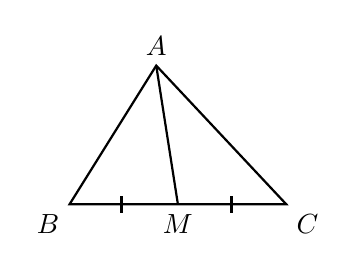
\begin{tikzpicture}[scale=1.1, >=stealth]
                \coordinate (A) at (1.0,1.6);
                \coordinate (B) at (0,0);
                \coordinate (C) at (2.5,0);
                \coordinate (M) at (1.25,0);
                
                \draw[thick] (A) -- (B) node[below left] {$B$} -- (C) node[below right] {$C$} -- cycle;
                \draw[thick] (A) -- (M) node[below] {$M$};
                \node[above] at (A) {$A$};
                
                % Ký hiệu bằng nhau
                \draw[thick] (0.6,-0.1) -- (0.6,0.1);
                \draw[thick] (1.87,-0.1) -- (1.87,0.1);
            \end{tikzpicture}
        \end{minipage}
        \hfill
        \begin{minipage}{0.55\textwidth}
            \[
            \boxed{AM^2 = \frac{2(AB^2 + AC^2) - BC^2}{4}}
            \]
        \end{minipage}
    \end{center}
    \textbf{Giải thích:}
    \begin{align*}
        \vec{AM} = \frac{1}{2}\left(\vec{AB} + \vec{AC}\right) &\implies \vec{AM}^2 = \frac{1}{4}\left(\vec{AB} + \vec{AC}\right)^2 \\
        &\implies AM^2 = \frac{1}{4}\left(AB^2 + AC^2 + 2\vec{AB}\cdot\vec{AC}\right) \\
        \text{Có: } 2\vec{AB}\cdot\vec{AC} &= AB^2 + AC^2 - BC^2 \\
        \implies AM^2 &= \frac{1}{4}\left(AB^2 + AC^2 + AB^2 + AC^2 - BC^2\right) \\
        &= \frac{2(AB^2 + AC^2) - BC^2}{4}
    \end{align*}
\end{enumerate}

\section*{II. KHÔNG GIAN}

\begin{enumerate}[label=\arabic*., leftmargin=*, itemsep=1.5em]
    % 21. Quy tắc hình hộp
    \item \textbf{Quy tắc hình hộp}
    \par Cho hình hộp $ABCD.A'B'C'D'$.
    \begin{center}
        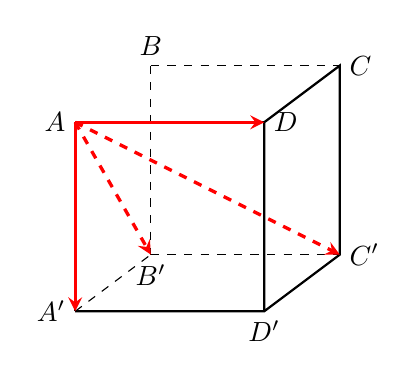
\begin{tikzpicture}[scale=1.2, >=stealth]
            % Tọa độ
            \coordinate (A) at (0,2);
            \coordinate (D) at (2,2);
            \coordinate (B) at (0.8,2.6);
            \coordinate (C) at (2.8,2.6);
            
            \coordinate (Ap) at (0,0);
            \coordinate (Dp) at (2,0);
            \coordinate (Bp) at (0.8,0.6);
            \coordinate (Cp) at (2.8,0.6);
            
            % Các nét đứt phía sau
            \draw[dashed] (B) -- (Bp);
            \draw[dashed] (B) -- (C);
            \draw[dashed] (Ap) -- (Bp);
            \draw[dashed] (Bp) -- (Cp);
            
            % Các nét liền phía trước
            \draw[thick] (Ap) -- (Dp) -- (Cp) -- (C) -- (D) -- (Dp);
            \draw[thick] (A) -- (Ap);
            \draw[thick] (A) -- (D);
            
            % Vectơ AB, AD, AA' (màu đỏ)
            \draw[->, red, very thick] (A) -- (D);
            \draw[->, red, very thick] (A) -- (Ap);
            \draw[->, red, dashed, very thick] (A) -- (Bp);
            
            % Vectơ đường chéo AC' (màu đỏ đứt nét)
            \draw[->, red, dashed, very thick] (A) -- (Cp);
            
            % Ghi nhãn đỉnh
            \node[left] at (A) {$A$};
            \node[right] at (D) {$D$};
            \node[above] at (B) {$B$};
            \node[right] at (C) {$C$};
            \node[left] at (Ap) {$A'$};
            \node[below] at (Dp) {$D'$};
            \node[below] at (Bp) {$B'$};
            \node[right] at (Cp) {$C'$};
        \end{tikzpicture}
    \end{center}
    Công thức hình hộp:
    \[
    \boxed{\vec{AB} + \vec{AD} + \vec{AA'} = \vec{AC'}}
    \]

    % 22. Trọng tâm của tứ diện
    \item \textbf{Trọng tâm của tứ diện}
    \par Cho tứ diện $ABCD$. Gọi $I$ là trung điểm $AB$, $J$ là trung điểm $CD$. Điểm $G$ thỏa mãn:
    \[
    \vec{GA} + \vec{GB} + \vec{GC} + \vec{GD} = \vec{0}
    \]
    Khi đó, $G$ được gọi là \textbf{trọng tâm của tứ diện $ABCD$}.
    \begin{center}
        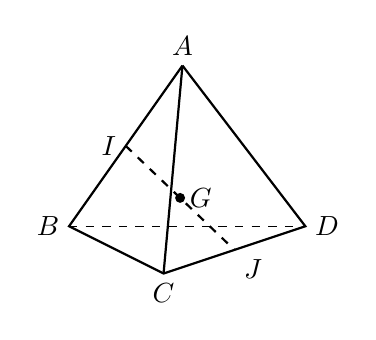
\begin{tikzpicture}[scale=1.2, >=stealth]
            \coordinate (A) at (1.2,2.2);
            \coordinate (B) at (0,0.5);
            \coordinate (C) at (1.0,0);
            \coordinate (D) at (2.5,0.5);
            
            % Cạnh đứt BD
            \draw[dashed] (B) -- (D);
            
            % Các cạnh ngoài liền
            \draw[thick] (A) -- (B) -- (C) -- (D) -- (A);
            \draw[thick] (A) -- (C);
            
            % Trung điểm I, J
            \coordinate (I) at (0.6,1.35); % trung điểm AB
            \coordinate (J) at (1.75,0.25); % trung điểm CD
            
            % Đoạn nối IJ
            \draw[dashed, thick] (I) -- (J);
            
            % Trọng tâm G
            \coordinate (G) at (1.175,0.8);
            \fill (G) circle (1.5pt) node[right] {$G$};
            
            % Ghi nhãn
            \node[above] at (A) {$A$};
            \node[left] at (B) {$B$};
            \node[below] at (C) {$C$};
            \node[right] at (D) {$D$};
            \node[left] at (I) {$I$};
            \node[below right] at (J) {$J$};
        \end{tikzpicture}
    \end{center}
    \textbf{Xác định vị trí của G:}
    \[
    \begin{cases}
        \vec{GA} + \vec{GB} = 2\vec{GI} \\
        \vec{GC} + \vec{GD} = 2\vec{GJ}
    \end{cases}
    \implies \vec{GA} + \vec{GB} + \vec{GC} + \vec{GD} = 2\left(\vec{GI} + \vec{GJ}\right) = \vec{0}
    \]
    \[
    \implies \vec{GI} + \vec{GJ} = \vec{0} \implies G \text{ là trung điểm của } IJ.
    \]
    \subsection*{II. Tính chất của trọng tâm tứ diện G}

\begin{enumerate}[label=\arabic*., leftmargin=*, itemsep=1.5em]
    % Tính chất 1
    \item Cho tứ diện $ABCD$, nếu $I, J, E, F, M, N$ lần lượt là trung điểm của các cạnh $AB, CD, AC, BD, BC, AD$ thì 3 đoạn thẳng $IJ, MN, EF$ cắt nhau tại trung điểm của mỗi đường, điểm đó chính là $G$.
    \begin{center}
        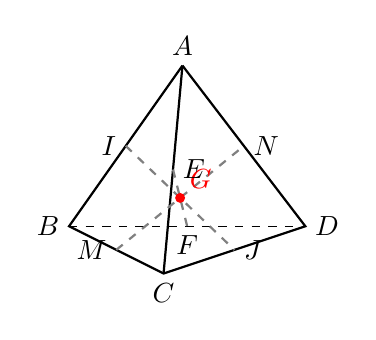
\begin{tikzpicture}[scale=1.2, >=stealth]
            \coordinate (A) at (1.2,2.2);
            \coordinate (B) at (0,0.5);
            \coordinate (C) at (1.0,0);
            \coordinate (D) at (2.5,0.5);
            
            \draw[dashed] (B) -- (D);
            \draw[thick] (A) -- (B) -- (C) -- (D) -- (A);
            \draw[thick] (A) -- (C);
            
            % Các trung điểm
            \coordinate (I) at (0.6,1.35); % AB
            \coordinate (J) at (1.75,0.25); % CD
            \coordinate (E) at (1.1,1.1); % AC
            \coordinate (F) at (1.25,0.5); % BD
            \coordinate (M) at (0.5,0.25); % BC
            \coordinate (N) at (1.85,1.35); % AD
            
            % Đoạn thẳng nối
            \draw[dashed, thick, gray] (I) -- (J);
            \draw[dashed, thick, gray] (E) -- (F);
            \draw[dashed, thick, gray] (M) -- (N);
            
            % Trọng tâm G
            \coordinate (G) at (1.175,0.8);
            \fill[red] (G) circle (1.5pt) node[above right] {$G$};
            
            % Ghi nhãn
            \node[above] at (A) {$A$};
            \node[left] at (B) {$B$};
            \node[below] at (C) {$C$};
            \node[right] at (D) {$D$};
            \node[left] at (I) {$I$};
            \node[right] at (J) {$J$};
            \node[right] at (E) {$E$};
            \node[below] at (F) {$F$};
            \node[left] at (M) {$M$};
            \node[right] at (N) {$N$};
        \end{tikzpicture}
    \end{center}

    % Tính chất 2
    \item Cho tứ diện $ABCD$, gọi $M$ là trọng tâm của tam giác $BCD$. Trên đoạn $AM$ lấy điểm $G$ sao cho $AG = 3GM$ thì $G$ chính là trọng tâm của tứ diện $ABCD$.
    \begin{center}
        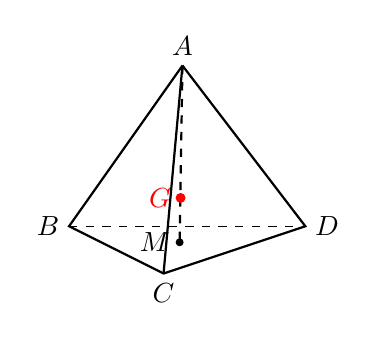
\begin{tikzpicture}[scale=1.2, >=stealth]
            \coordinate (A) at (1.2,2.2);
            \coordinate (B) at (0,0.5);
            \coordinate (C) at (1.0,0);
            \coordinate (D) at (2.5,0.5);
            
            \draw[dashed] (B) -- (D);
            \draw[thick] (A) -- (B) -- (C) -- (D) -- (A);
            \draw[thick] (A) -- (C);
            
            % Trọng tâm M của BCD
            \coordinate (M) at (1.17,0.33);
            \fill (M) circle (1.2pt) node[left] {$M$};
            
            % Đoạn AM
            \draw[dashed, thick] (A) -- (M);
            
            % G trên AM
            \coordinate (G) at (1.18,0.8);
            \fill[red] (G) circle (1.5pt) node[left] {$G$};
            
            \node[above] at (A) {$A$};
            \node[left] at (B) {$B$};
            \node[below] at (C) {$C$};
            \node[right] at (D) {$D$};
        \end{tikzpicture}
    \end{center}
    \textbf{Giải thích:}
    \[
    \vec{GA} + \vec{GB} + \vec{GC} + \vec{GD} = \vec{0} \Leftrightarrow \vec{GA} + 3\vec{GM} = \vec{0} \quad (\text{do } M \text{ là trọng tâm } \triangle BCD)
    \]
    \[
    \Leftrightarrow \vec{GA} = -3\vec{GM}
    \]

    % Tính chất 3
    \item Cho tứ diện $ABCD$, gọi $M_1, M_2, M_3, M_4$ lần lượt là trọng tâm của các tam giác $BCD, CDA, DAB, ABC$. Khi đó các đoạn $AM_1, BM_2, CM_3, DM_4$ cắt nhau tại cùng 1 điểm, điểm đó là $G$, là trọng tâm tứ diện $ABCD$.

    % Tính chất 4
    \item Nếu $G$ là trọng tâm tứ diện $ABCD$ thì với $S$ là điểm bất kỳ, ta luôn có:
    \[
    \vec{SA} + \vec{SB} + \vec{SC} + \vec{SD} = 4\vec{SG}
    \]
    \textbf{Chứng minh:}
    \[
    \begin{cases}
        \vec{SA} = \vec{SG} + \vec{GA} \\
        \vec{SB} = \vec{SG} + \vec{GB} \\
        \vec{SC} = \vec{SG} + \vec{GC} \\
        \vec{SD} = \vec{SG} + \vec{GD}
    \end{cases}
    \implies \vec{SA} + \vec{SB} + \vec{SC} + \vec{SD} = 4\vec{SG} + \underbrace{(\vec{GA} + \vec{GB} + \vec{GC} + \vec{GD})}_{\vec{0}} = 4\vec{SG}
    \]
\end{enumerate}
\end{document}